\chapter*{Contexte : Colonie d'abeilles et Complexité, Biologie et Systèmes Complexes}
\addcontentsline{toc}{chapter}{Contexte : Colonie d'abeilles et Complexité, Biologie et Systèmes Complexes}
\chaptermark{Contexte : Colonie d'abeilles et Complexité, Biologie et Systèmes Complexe}
	\label{sectionBio}
	
	Les insectes sociaux sont depuis longtemps étudiés pour leurs capacités complexes à se répartir dynamiquement le travail, sans l'aide d'un contrôle central. Ce chapitre présente tout d'abord les principales notions de complexité, et donne plusieurs exemples de phénomènes complexes que l'on peut retrouver dans la vie d'une colonie d'abeilles. Nous verrons dans le chapitre suivant quelques modèles Multi-Agents présents dans la littérature servant à modéliser ces systèmes.

	
		\subsubsection{Systèmes complexes}
		
			Il n'existe à ce jour pas de définition précise de ce qu'est un système complexe \cite{heylighen_complexity_2008}, du fait de l'étendue vertigineuse des domaines et cas d'applications touchés. Ils sont souvent composés d'une multitude de composants hétérogènes, ni communiquant que très peu entre eux, liés par leurs interactions mutuelles dans un tout, le système complexe. Un système complexe est toutefois un bon exemple de l'adage "Le tout vaut plus que la somme des parties" d'Aristote \cite{edmonds_what_1999}. En effet, nous retrouvons souvent dans la littérature les notions de chaos, d'interactions locales et d'imprévisibilité. Un système complexe ne peut pas être anticipé par le calcul, le seul moyen d'en connaitre l'état futur et de l'observer. Ceci est notamment lié à leur propriétés émergentes : nous parlons d'émergence lorsque des comportements apparaissent grâce à des interactions entre différents composants, et que ces comportements sont absent lorsque ces composants sont étudiés séparément. Les propriétés émergentes sont le plus souvent imprévisibles, donnant ainsi cette propriété aux systèmes complexes. Toutes ces émergences de comportements et boucles de rétroactions génèrent un système qui peut être dit chaotique. Suivant les théories du chaos, ou "l'effet papillon", ces systèmes ont alors hautement imprévisible et de légère variation de paramétrage ou de conditions initiales peuvent avoir de grande conséquences sur le comportement global du système : "petit changement, grandes conséquences". De cette manière, nous pouvons imaginer un système peuplé de nombreuses entités aux caractéristiques bien différentes, mais qui interagissent entre-elles via diverses boucles de rétroactions. C'est ainsi que l'ordre peut émerger du chaos. Lorsque le système complexe s'organise indépendamment, sans intervention extérieure, et obtient ordre et structure, nous parlons d'auto-organisation.
			
			Clés dans cette organisation, les interactions multiples entre les différentes composantes du système font le plus souvent émerger des boucles de rétroactions.
			
			\begin{figure}
			\centering
			\includegraphics[width=0.8\textwidth]{Pictures/Figures/RetroActionsExemples.png}
			\caption{Boucles de rétroactions simplifiées du fonctionnement d'une bombe nucléaire à fission, ou bombe A (à gauche) et de l'équilibre hydrostatique du soleil (à droite). Un lien bleu se terminant par une flèche indique un renforcement, par exemple, la Pression au centre du Soleil vient augmenter son Rayon. Un lien rouge se terminant par un cercle indique une réduction : la Gravité à tendance à réduire le Rayon du soleil, en appliquant une force constante de toute part.}
			\label{retroActions}
			\end{figure}
		
		Une boucle de rétroaction est un processus qui lie un effet à sa propre cause. En électronique, cela consiste à brancher la sortie d'un composant à l'une de ses entrées. Les boucles de rétroaction se présentent sous deux formes, les rétroactions positives et négatives. Les boucles de rétroactions positives consistent en des phénomènes de renforcement, d'accélération. Nous parlons alors dans le langage courant de "cercle vicieux ou vertueux". Une bombe nucléaire à fission fonctionne avec ce principe, une fission va en déclencher plusieurs autres, qui vont à leurs tours en déclencher bien d'autres, sous une forme d'escalade de la violence exponentielle. La Figure \ref{retroActions} illustre cet exemple, montrant l'amplification constante de la réaction, où chaque fission va augmenter le nombre de fissions réalisées par la bombe, par le biais d'émission de neutrons. Sans autre mécanisme pour les réguler, ce sont des phénomènes très transitoires. Les autoroutes de fourmis, de leur côté, utilisent un mécanisme de renforcement pour marquer les pistes avec des phéromones. Cette boucle de rétroaction positive est régulée par l'évaporation de ces phéromones, qui viennent contrer un potentiel emballement du système. 
		
		les boucles de rétroaction négatives consistent en mécanismes régulateurs, stabilisant un système vers un équilibre. Nous pouvons en trouver de toutes sortes, sous bien des formes. Le soleil par exemple, voit sa forme maintenue par une boucle de rétroaction négative, à ce qui est appelé un équilibre hydrostatique \cite{haubold_analytic_1992} : lorsque son cœur réalise la fusion nucléaire, il crée une immense force en son centre, le faisant s'étendre. Le soleil gonfle alors et fait ainsi baisser la pression en son centre, le nombre de fusion est alors légèrement réduit. La force poussant le soleil à s'étendre est alors contrée par la gravité, le poussant de toute part vers son centre. Le soleil s'effondre sur lui même ! Mais du même temps, la pression en son centre remonte, les fusions reprennent de plus belle et il gonfle à nouveau : le soleil danse légèrement autour de son point d'équilibre. La Figure \ref{retroActions} illustre ces interactions, et montre la rétroaction entre la Pression et le Rayon du soleil : augmenter la Pression augmente le Rayon du soleil, noté par une flèche bleu. Or, augmenter le Rayon réduit la Pression, noté par un lien rouge se terminant par un cercle.
			
			Pour récapituler, un système complexe est composé d'une multitude de composants interagissant mutuellement avec des communications limitées. Ils sont imprévisibles et voient la plupart de leur propriété émerger des interactions entre composants, sous la forme de boucle de rétroactions.
			
			Un bel exemple de tels systèmes auxquels nous sommes soumis tous les jours est le climat. De faibles interactions qui peuvent paraitre insignifiantes ont de grosses répercussions sur le système dans son ensemble. Nous augmentons d'un demi degré la température des océans et ce sont les courants marins, les vents et tempêtes, les chaines alimentaires et bien d'autres qui se dérèglent. Augmenter de quelques points le pourcentage de gaz à effet de serre dans l'atmosphère et le circuit s'emballe et réchauffe le tout, augmentant la fréquence d'événements violents etc \cite{allen_2018_2018}. Une grande quantité d'entités, jusqu'à l'échelle moléculaire, vont interagir entre elles, faisant varier leurs températures, leurs pressions, leurs absorptions et réflexions de la lumière, altérant par la même occasion le climat sur une échelle planétaire, affectant jusqu'à notre mode de vie. 
						
			Nous allons maintenant constater en quoi une colonie d'abeilles est un bon représentant de la grande famille des systèmes complexes.
			
			

	
		\subsubsection{Abeilles et Systèmes complexes}		
			Une colonie classique d'abeilles domestiques \textit{Apis Melifera} héberge en moyenne quelques dizaines de milliers d'individus, 50 000 est un nombre qui revient souvent. Tous ces individus ont des besoins en nourritures et en eau, mais l'attention au couvain, regroupant tous les stades de vie de l'abeille avant sa phase adulte, demande un tout autre niveau d'attention : nourriture spéciale, température précise, cellules de cires propres etc. Tous ces besoins créent une chaine logistique impressionnante, que des apiculteurs observent depuis des milliers d'années \cite{oldroyd_domestication_2012}. En effet, les abeilles (et bien d'autres insectes sociaux) arrivent à survivre et même à s'épanouir sans aucun contrôle central, aucun individus spéciaux chargés du management ou de la surveillance des stocks. Des rôles ont été créés pour classer les différents maillons de cette chaîne, dont nous allons décrire les principaux \cite{winston_biology_1991, winston_role_1991, seeley_age_1991}. 
			
			Emblématique de la colonie d'abeilles et présentant des différences physiques notables, la Reine, plus grande que les autres abeilles, est chargée de pondre à une vitesse ahurissante : près d'un œuf par minute en moyenne sur toute sa vie. Elle est en permanence entourée d'une "cour royale", d'autres abeilles qui viennent la lécher de tous côtés, attirées par ses phéromones puissantes. Elles vont ensuite répandre les phéromones royales dans toutes la colonie, permettant ainsi à l'ensemble de la colonie de sentir la présence de la reine. Souvent ces abeilles sont des nourrices, elles sont chargées de nourrir le couvain. De vraies cuisinières, elles parcourent la ruche à la recherche de miel et de pollen afin de concocter un liquide calorifique dont les larves se nourrissent. Parfois, une recette alternative encore plus riche, la gelée royale, est donnée à des larves spécialement sélectionnées pour devenir de nouvelles reines.
			
			Les larves sont des systèmes digestifs autonomes. Elles ingurgitent de grandes quantités de nourriture par rapport à leur poids, pour assurer leur croissance rapide, et leur permettre de devenir par la suite de solides ouvrières. La reine pond des œufs, qu'elle dépose au fond de cellules. Ces cellules doivent être bâties par des ouvrières cirières, et nettoyées, la reine ne pond jamais dans une cellule sale. Une fois pondu, un œuf va mettre trois jours pour évoluer en larve, puis consommer son mélange de miel et de pollen pendant les six jours que représentent l'état de larve, puis va devenir une nymphe, étape importante où la larve va se métamorphoser progressivement en sa forme finale, une abeille adulte, 21 jours après la ponte. Dès qu'une larve passe au stade de nymphe, elle est repérée par une ouvrière cirière qui va méthodiquement operculer la cellule : créer une sorte de toit afin de celer la nymphe qui devra ouvrir sa cellule elle même, dans ses premières heures d'adulte, à l'aide de ses nouvelles mandibules.
			
			Pour que toute cette croissance se passe bien, la température du couvain doit être exactement de 35°C. Un écart de l'ordre du demi degré peut engendrer des pertes colossales, et mettre la colonie en péril. Certaine abeilles effectuent alors des tâches de thermo-régulation, lorsqu'il fait trop chaud ou trop froid. 

	\begin{wrapfigure}{r}{0.5\textwidth}
	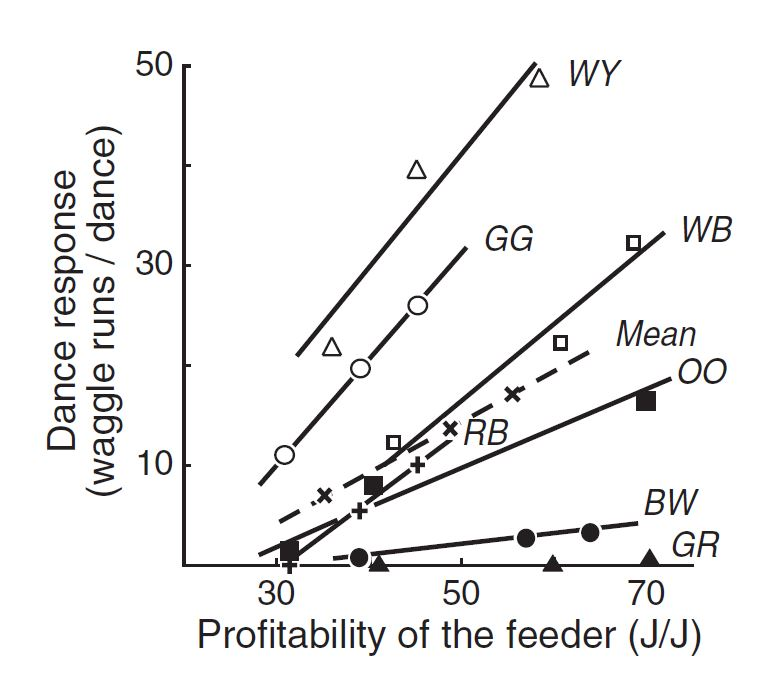
\includegraphics[width=0.45\textwidth]{Pictures/Graphs/SeeleyWaggles.JPG}
	\caption{Tiré des travaux de T.D.Seeley \cite{seeley_wisdom_1995}. En abscisses la profitabilité de la source, et en ordonnées le nombre de danses répétées par chaque abeilles après être rentrée à la ruche. 7 butineuses ont été observées après avoir récolté du nectar sur une source contrôlée, leurs danses ont été enregistrées. Ils ont ensuite montré que le nombre de danse et leurs durées sont directement liés à la teneur en sucre de la source.}
	\label{SeeleyWaggles}
	\end{wrapfigure}
			
			Les abeilles sont surtout célèbres pour leur butinage, rôle tenu par les "butineuses". Celles-ci sélectionnent les meilleurs sites de ressources sur une surface dépassant souvent les 100km² \cite{seeley_wisdom_1995} et ramènent nectar et pollen à la colonie. Certaines abeilles vont spontanément quitter la ruche sans destination, dans le seul but de trouver une nouvelle source de nectar. Ces butineuses sont appelées des "scouts", ou des "éclaireurs". Elles repèrent les fleurs grâce à leurs immenses yeux sensibles aux ultra-violets, que les fleurs ont appris à bien réfléchir dans une co-évolution avec les pollinisateurs \cite{thompson_concepts_1989}. Une fois sur une source de nectar, il est temps d'en juger la qualité. L'abeille va récolter le nectar, et estimer sa teneur en sucre \cite{seeley_wisdom_1995}. Si cette teneur lui convient, elle va rentrer à la colonie et commencer la troisième étape, le point clé, le recrutement. Mais avant ceci, une fois rentrée, la butineuse cherche une "receveuse" : une fois trouvée, elle lui donne une partie de sa charge de nectar. Les butineuses donnent ainsi leur récolte à trois ou quatre receveuses. Ensuite, elles viennent déposer leurs ballots de pollen dans des cellules proches du couvain, puis repartent. 
	
	Avant de décoller, l'abeille recruteuse va se mettre à danser la \textit{"Waggle Dance"}, en forme de 8. Cette danse a un objectif double. Le premier consiste à communiquer la position de la source de nectar par rapport au soleil ainsi que sa distance à la ruche, pour permettre aux autres de la retrouver. Le second est plus indirect : plus la source est sucrée et proche, et donc profitable, plus l'abeille va danser longtemps, et même répéter la danse dans plusieurs endroits de la ruche. Une danse plus longue offre plus de temps à d'autres abeilles de venir la suivre et apprendre la position de cette nouvelle source. Ainsi, plus la source est profitable, plus la recruteuse va communiquer la position à de nombreuses butineuses. La Figure \ref{SeeleyWaggles} est tirée des travaux de T.D.Seeley \cite{seeley_wisdom_1995} et illustre empiriquement que les abeilles dansent de manière plus instense pour des sources plus sucrées.
			
			Dans le même temps, les receveuses vont déposer le nectar reçu dans des cellules, toujours très hautes sur le cadre. Certaines iront aussi tasser les ballots de pollen dans leurs cellules, afin de ne pas perdre de place. Le nectar est alors prêt à subir ses transformations pour devenir du miel. Certaines abeilles vont alors venir "cracher" sur le nectar, afin d'y déposer leurs enzymes qui feront le travail de transformation. Elles y déposent du même coup une substance antiseptique, s'assurant ainsi que le miel ne sera pas contaminé par de mauvaises bactéries ou virus (c'est en partie ce qui lui confère ses propriétés médicales). Ensuite, pendant ce travail d'enzymes, des "ventileuses" viendront se placer au dessus du miel et battre frénétiquement des ailes. Elles ajustent ainsi l'hygrométrie du miel, l'amenant très précisément a 15\% d'humidité, parfait pour la conservation.
			
			Toutes ces ouvrières sont sœurs ou demi-sœurs. Elles ont la plupart du temps toutes la même mère, mais pas forcément le même père. Au moment de la ponte, la reine "choisi" de féconder ou non son œuf. Les cellules où sont pondus les mâles sont plus grandes que celles des femelles, l'hypothèse la plus répandue est que les cellules plus petites des femelles viennent comprimer l'abdomen de la reine, provoquant ainsi la fécondation, sans décision au moment de la ponte. Par la magie de la biologie, un œuf non fécondé donnera un mâle, un œuf fécondé donnera une femelle. Les mâles ont une vie très particulière : ils sont incapables de quoi que ce soit, ni de se laver, ni de se nourrir seuls, et ne font rien dans la colonie. Dès que la situation se gâte et que les ressources se font rares, ce sont les premiers à être chassés de la colonie. Reconnaissable à leurs immenses yeux, ils ne sont bon qu'à un chose, s'envoler au bon moment vers un point de rencontre défini (on ne sait pas trop comment), localiser une reine et la féconder. Ils meurent instantanément après l'acte (globalement leur intérieur explose). Une reine est ainsi fécondée par une dizaine de mâles et va garder leurs semences dans sa spermathèque et s'en servir tout au long de sa vie.
			
			Nous allons désormais nous intéresser plus en détails à ces nombreux mécanismes de contrôles comme celui-ci. Comment les abeilles parviennent à savoir quoi faire, sans personne pour diriger le tout.
			
		\subsubsection{Auto-Organisation de la Colonie}
			Afin d'assurer le bon fonctionnement et l'épanouissement de la colonie, chaque individu la composant doit effectuer un certain nombre de tâches lorsqu'elles sont nécessaires, et sans aucun contrôle central. Par exemple, personne pour surveiller la température et assigner une équipe à la régulation de la température pendant un certain temps. Nous parlons alors d'auto-organisation. Chaque individu utilise ses perceptions locales pour savoir quel travail réaliser, ainsi nous parlons aussi d'allocation du travail. Les quelques mécanismes complexes d'auto-organisation (et leurs boucles de rétroactions) que nous allons aborder sont les suivants (il en existe bien d'autres, et surement une majorité dont nous ignorons pour l'instant jusqu'à l'existence) :
			
			
			\begin{itemize}
				\item La thermorégulation : la température est maintenue précisément à 35°C au niveau du couvain.
				\item La sélection des meilleures sources de nourritures par les butineuses par le biais de leur mécanisme de recrutement.
				\item La régulation de l'âge du premier butinage en fonction des demandes du couvain, les variations de vitesses de vieillissement chez les ouvrières.
			\end{itemize}

			\subsubsection{Thermorégulation}	
			
			Lorsqu'il fait légèrement trop chaud nous trouvons des abeilles thermo-régulatrices : elles battent des ailes sur le couvain et/ou au niveau de la sortie de la ruche pour créer un courant d'air et rafraichir la ruche. Certaines vaporisent même de l'eau dans la ruche pour aider à faire chuter la température. Lorsqu'il fait froid, les abeilles se resserrent progressivement au dessus du couvain, afin de créer ce qui est appelé la "grappe" et tenir le couvain au chaud, grâce à leurs corps. Si leur simple présence ne suffit plus, elles peuvent actionner certains de leurs muscles afin de générer un peu plus de chaleur, ce qui arrive pendant l'hiver, phase critique pour la colonie. Si la grappe est trop petite pour recouvrir l'ensemble de couvain, alors une bonne partie de ce dernier, celui en périphérie qui n'aura pas été protégé par les adultes, va mourir, on l'appelle alors le "couvain refroidi".		
			Un des points clés de cette capacité est que chaque individu a des "tolérances" légèrement différentes. Une diversité qui provient notamment de la présence des ces fameuses "demi-sœurs", dont nous avons parlé juste avant. J. Jones et.al. \cite{jones_honey_2004} ont montré que a capacité des abeilles à réguler la température est liée à cette diversité génétique. En effet, pour que la colonie régule correctement, il est important d'éviter des mouvements de foules à l'échelle de la colonie, afin de ne pas osciller entre trop chaud et trop froid en permanence. La diversité génétique modifie légèrement les seuils des tolérances des abeilles, qui vont alors progressivement réguler la température. Lorsque la température sera légèrement trop haute, seules certaines abeilles ventileront, les autres, de part leurs tolérances plus élevées, ne vont pas participer. Ainsi, si l'action des premières est suffisante, la température revient doucement au bon niveau. Si la température continue de monter, alors de plus en plus d'abeilles la verront atteindre leur seuil de tolérance, et se joindront à l'effort.
			
			De cette manière, chaque individu mesure et juge la température actuelle de la colonie, et prends alors la décision de réchauffer, refroidir, ou réaliser d'autres devoirs. Sa position dans la ruche et sa sensibilité personnelles vont entrer en compte dans cette décision. Ainsi, par l'action autonome de chacun des individus, la température du couvain ne s'écarte jamais plus d'un degré de 35°C. La colonie voit a toujours un nombre optimal d'individu régulant la température, permettant de répondre parfaitement au besoin sans délaisser les autres tâches.
			
			\subsubsection{Sélection des meilleures sources de nectar}
			Lors de la collecte du nectar, les butineuses sont très sélectives et préfèrent les nectars aux hautes teneurs en sucres sur des fleurs placés le plus proche possible de la ruche. La colonie utilise donc un système de recrutement, presque de recommandation, afin d'allouer ses effectifs de butineuses de manière optimale et dynamique, préférant les sources proches et nutritives.
			Une fois recrutées, les nouvelles butineuses vont se rendre à la source et répéter le processus : collecter, juger, rentrer et parfois recruter. Là encore, la diversité est clé : des abeilles moins portées sur la communication vont passer moins de temps à recruter, afin de maximiser le temps de butinage. En effet, il y a tout de même des dizaines de milliers de bouches à nourrir ! De plus, certaines butineuses sont moins difficiles que d'autres, elles vont donc communiquer des sources de faible qualité et y maintenir un faible contingent. Ce contingent alors moins utile dans l'immédiat sert de surveillance, car les teneurs en sucres des différents nectars peuvent fortement varier selon les saisons mais aussi pendant les périodes de la journée. Une source de faible qualité peut alors devenir une source extrêmement intéressante en quelques heures. Le groupe alors déjà présent peut observer ce changement et déjà danser sur une zone bien définie, proche de l'entrée, appelée la "piste de dance", pour avertir les autres, gagnant ainsi un temps précieux de re-découverte de la source mais aussi le temps d'amorcer une réponse conséquente. Gagner du temps sur une réaction exponentielle est toujours extrêmement précieux. C'est en effet une boucle de rétroactions positive, plus il y a d'abeilles à apprécier la source, plus il y aura de recruteuses, augmentant ainsi encore le nombre de recruteuses par la suite.
			
			la diversité génétique fait ici effet de régulation, et permet d'ajuster le butinage en un savant équilibre entre exploration et exploitation. Il est certes important de ramener d'énorme quantité de nourriture à la colonie, mais avoir la totalité de ses effectifs sur une même source présente des risques. Les abeilles "scouts", ainsi que les "moins difficiles" citées plus tôt vont alors permettre de maintenir l'exploration et la découverte de nouvelle ressources à un niveau sécurisant, multipliant les opportunités.
			
		\subsubsection{Phéromones et Physiologie}
			\label{subsubPhysio}
			L'auto-organisation de la colonie ne se joue pas que dans les perceptions, la colonie s'appuie sur des mécanismes indirects, long-termes, physiologiques, qui prennent place grâce à différentes hormones et phéromones.  Nous étudions ici en détail l'importance physiologique des glandes hypopharyngiennes (GH) et de la Corpora Allata. C'est ce mécanisme qui nous intéresse tout particulièrement dans ce manuscrit. La Corpora Allata permet aux adultes de sécréter une hormone appelée Hormone Juvénile(HJ). Cette hormone est retrouvée en grande quantité chez les butineuses, et en faible quantité chez les nourrices. Les GH permettent aux abeilles s'occupant du couvain de transformer le pollen et le nectar en une substance riche destinée aux larves. Elles permettent aussi aux butineuses de traiter chimiquement le nectar, le rendant utilisable pour les nourrices, transformable en miel et même consommable directement par les autres adultes. Or, ces deux comportements sont incompatibles, les GH subissent une modification physiologique pour effectuer l'une ou l'autre de ces fonctions. De plus, les abeilles (ainsi que d'autres insectes sociaux) emploient différentes phéromones pour parvenir à s'épanouir. Ces phéromones peuvent être séparées en deux catégories : les phéromones modificatrices, et les phéromones incitatrices. Les phéromones modificatrices, comme leur nom l'indique, viendront modifier la physiologie des individus : ce sont elles qui sont notamment responsable de la modification des propriétés des GH que nous venons d'aborder. Les phéromones incitatrices quant à elles viendront déclencher des comportements, sans altération physique sur les agents. Ainsi, nous pouvons voir les phéromones incitatrices comme ayant un effet très court terme, et les phéromones modificatrices un effet très long terme. Par exemple, lors d'une attaque, les premières abeilles témoins viendront émettre une phéromone d'alarme très volatile, qui aura pour effet de faire sortir une grande quantité d'abeilles de la ruche pour servir de renfort. Cette phéromone incitatrice augmente aussi fortement l'agressivité des abeilles. Fait étonnant, d'après certains apiculteurs, cette phéromone aurait parfois une odeur proche de la banane !
			
			
			
			
			\begin{figure}
				\includegraphics[width=\textwidth]{Pictures/Figures/PhModificatrices.png}
				\caption{Synthèse des connaissances simplifiées et schématisées des phéromones modificatrices au sein de la colonie. Un lien bleu se terminant par une flèche indique un renforcement, par exemple, l'Ocimene vient augmenter la concentration d'Hormone Juvénile des adultes. Un lien rouge se terminant par un cercle indique une réduction : le 9-ODA vient réduire, ou inhiber les Ovaires des ouvrières.}
				\label{phMod}
			\end{figure}	
			
			La Figure \ref{phMod} schématise les interactions entre phéromones modificatrices, hormones et glandes, ainsi qu'entre différents individus de la colonie, que nous allons décrire dans cette partie. Nous avons pu construire ce modèle simplifié des phéromones modificatrices avec des collègues biologistes de l'INRAE, à Avignon \textit{Comment citer Yves et Cedric ici ?}. Cette Figure présente les trois principales phéromones modificatrices connues à ce jour. À gauche, les phéromones E-$\beta$-Ocimene (que nous appellerons désormais Ocimene pour plus de clarté) sont majoritairement émisent par de très jeunes larves (moins de 3 jours). Ces phéromones réduisent le développement ovarien des ouvrières (représenté par un lien rouge sur la figure) et déclenche une forte hausse de butinage de pollen de la part des butineuses, qui se concentrent habituellement sur le nectar \cite{maisonnasse_e-b-ocimene_2010}. Ensuite, le 9-ODA, un des composants des puissantes phéromones de reine, ralenti lui aussi le développement ovarien des butineuses mais réduit aussi les concentrations en Hormone Juvénile (HJ) chez les ouvrières. Une hypothèse répandue est de considérer que l'HJ sécrétée par la Corpora Allata permet d'altérer le fonctionnement des GH, dictant ainsi leur utilité pour les nourrices ou les butineuses \cite{robinson_colony_1998}. Typiquement, la transition de nourrice à butineuse se fait en une vingtaine de jours. La colonie suit ce qu'on appelle le Polyéthisme d'Âge : les adultes ayant le même âge réalisent les mêmes activités. Or, il a été montré que ce polyéthisme est souple, et que dans les bonnes conditions, une abeille peut aller butiner dès ses 5 jours, au lieu de la vingtaine habituelle. Ce mécanisme est lié à une phéromone, émise par toute la colonie, l'Ethyle Oléate (EO). La réduction d'HJ provoquée par l'Ocimene et le 9-ODA permet donc de maintenir ces ouvrières à une physiologie de nourrices.
			
			 L'Ethyle Oleate est retrouvée majoritairement sur le couvain et la reine, elle est aussi retrouvée chez les butineuses. Lorsque cette phéromone est injectée en grande quantité à des abeilles adultes, il a été montré que celles-ci arrêtent le butinage et voient leur taux d'HJ diminuer. L'Ethyle Oléate n'est pas une phéromone volatile, elle est majoritairement transmise par contact, principalement lors d'échange de nourriture et de nettoyage mutuel : lorsqu'une abeille en nettoie une autre, ou lorsqu'une nourrice nettoie une larve. Elle serait aussi transmissible sur de courtes distances par évaporation. On observe sur la Figure \ref{phMod} que l'EO favorise le développement des GH, qui elles même réduisent et son altérées par l'HJ. Nous y observons aussi que l'EO ralenti le développement ovarien des ouvrières. Dans le cas classique du polyéthisme d'âge, les jeunes abeilles effectuent un travail de nourrices, et les plus âgées butinent. Mais, comme nous venons de le voir, une nourrice peut accélérer sont vieillissement, et une butineuse peut même l'inverser, afin de s'adapter aux besoins changeant de la colonie. C'est pour ceci que nous parlerons ici d'Age Physiologique, opposé à l'âge réel. Une abeille avec un faible âge physiologique possède les GH nécessaires aux nourrices, et les plus âgées physiologiques possèdent les GH et les muscles nécessaires au vol et au butinage.
			
		\subsubsection{Conclusion}
			
		Dans ce chapitre nous avons présenté le concept de système complexe, en quoi une colonie d'abeilles en est un représentant tout en réalisant un rapide état de l'art sur les connaissances biologiques de ces insectes sociaux. Régulation de la température, adaptation de la physiologie en fonction des besoins, allocation de travailleurs sur différentes sources de nourritures en fonction de leur profitabilité sont les points que nous avons abordés, mais la colonie en contient bien d'autres, et beaucoup restent encore à être découvert. Toute cette auto-organisation, sans aucun contrôle central, représente un grand intérêt de recherche, pour comprendre leurs méthodes, les reproduire et essayer d'en extraire les principes pour des applications scientifiques et technologiques. Le chapitre suivant aborde donc les différents modèles informatiques utilisés pour simuler de tels systèmes, et présente quelques exemples d'application de ces-derniers pour des simulation.